%!TEX root = ../main.tex

\chapter{UMAP} 

\label{UMAP} 

%----------------------------------------------------------------------------------------

% N O T I Z E N
% Wirkung des Funktors beschreiben \cite{Posada}
% Bisher: Daten -> metr. R�ume -> fuzzy simplicial sets
% Ziel:   Daten -> metr. R�ume -> VR complex

% T E X T B A U S T E I N E
% 

%----------------------------------------------------------------------------------------
%----------------------------------------------------------------------------------------

% \section{Einleitung}
In diesem Kapitel werden wir die aus \ref{Grundlagen} erlangten Grundlagen verwenden um 
eine geeignete topologische Repr�sentation unserer Daten $X=\seqx$ zu erlangen. Eine �hnliche 
Repr�sentation werden wir von einem $d$-dimensionalen Raum $(d \ll D)$ betrachten, um dann mit einem geeigneten 
Begriff des Abstandes der beiden Repr�sentationen die niedrigdimensionale Repr�sentation der 
hochdimensionalen anzupassen. Dies wird uns zum UMAP Verfahren f�hren. 
% TODO: Erg�nzungen hier erw�hnen oder in \ref{Implementierung}?

%----------------------------------------------------------------------------------------

\section{Topologische Repr�sentation}
Blabla bla

%-----------------------------------

\subsection*{Fluch der Dimensionen}
% Zitiere Bengio 2007
Ein kritischer Punkt beim analysieren hochdimensionaler Daten ist der sogenannte Fluch der Dimensionen.
Was das bedeutet und wie das UMAP Verfahren macht um diesen zu vermeiden werde ich im Folgenden kurz erkl�ren.
Unter dem Fluch der Dimensionen versteht man.


Siehe Abbildung \ref{fig:Curse}

\begin{figure}
	%\centering
	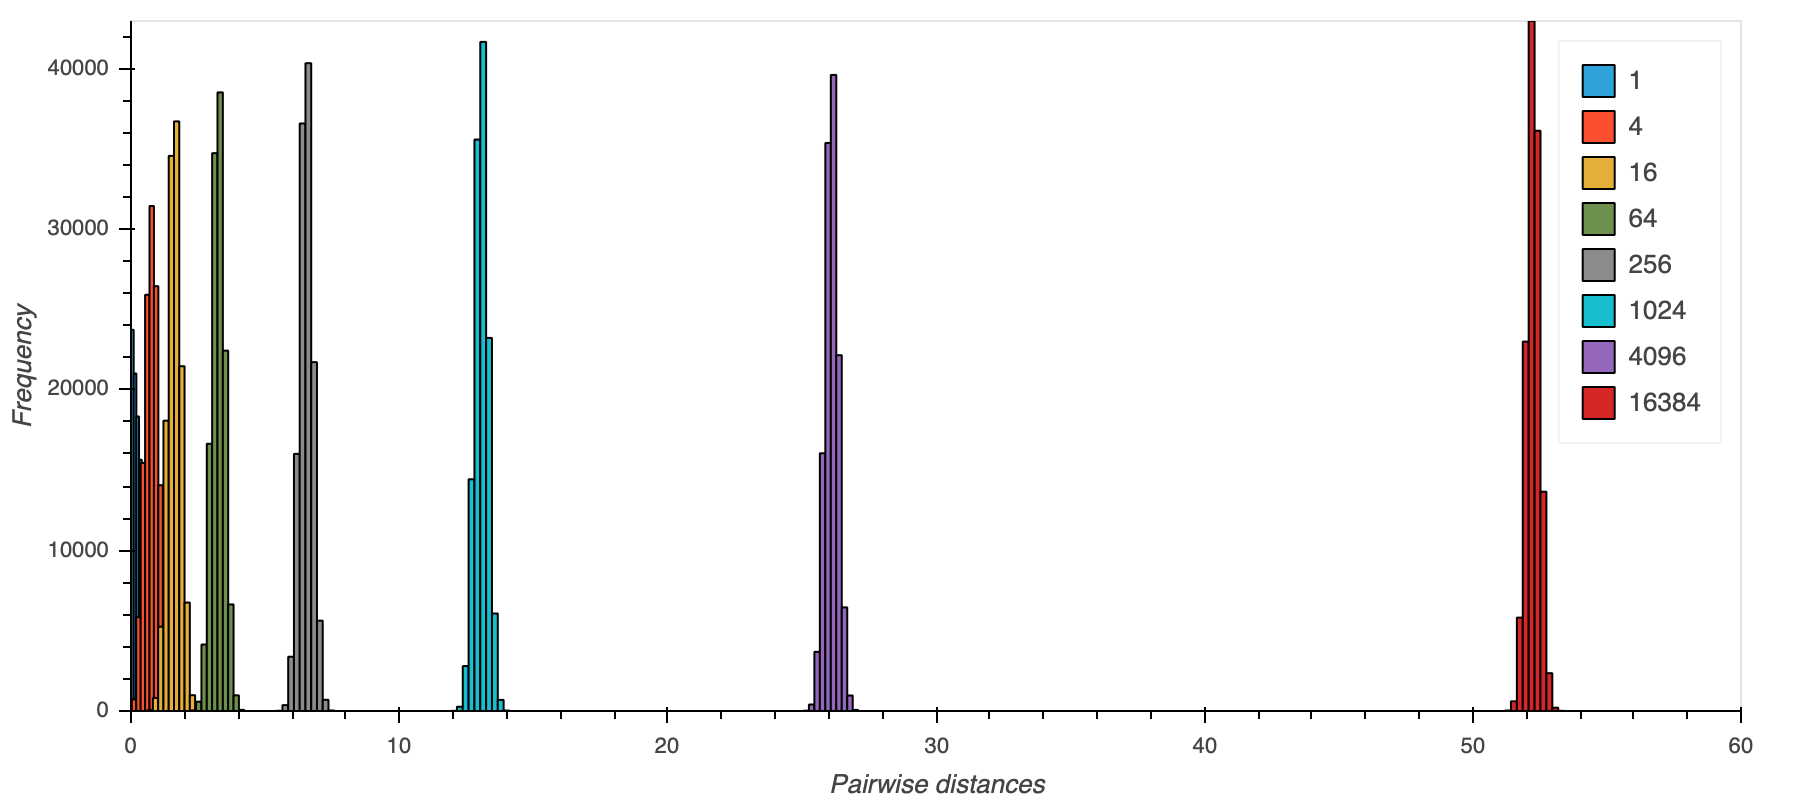
\includegraphics[width=400px, height=178px]{Figures/pairwise_dist}
	%\decoRule
	\caption[Durchsch. Distanz]{Paarweise Distanzen von $N=500$ zuf�llig gleichverteilten Punkten im $R^D$.}
	\label{fig:Curse}
\end{figure}

%-----------------------------------

%----------------------------------------------------------------------------------------

\section{Erg�nzungen}

% Wenn VR Komplex ausreichend, betrachte nur 1-Skelet und berechne Homologie darauf.
% Siehe Oudot s.48, funktioniert noch nicht f�r Filtrationen. 

